\documentclass[10pt,letterpaper]{article}
\usepackage[margin=0.75in]{geometry}
\usepackage[utf8]{inputenc}
\usepackage[T1]{fontenc}
\usepackage[stretch=10]{microtype}
\usepackage{hyperref}
\usepackage{tgpagella}
\usepackage{enumitem}
\usepackage{indentfirst}
\usepackage{graphicx}
\graphicspath{ {./images/} }
\pagestyle{empty}
\begin{document}

\begin{center}
\huge 
\textbf {K U VARUNKUMAR}
\end{center}


\hrule
\vspace{1.0em}
\begin{description}
\item Basava Krupa, \hfill Contact:91-8310604858
\item  Pragathi Nagar, \hfill e-mailid:astrovarun8@gmail.com 
 \item Kinnal Road,
\item  Koppal-583231,
\item Karnataka
\end{description}

\hfill 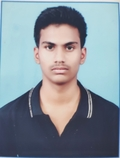
\includegraphics{varun}

\vspace{5.0em}


\hrule
\subsection*{OBJECTIVE}
   I am interested to work in the field of  Machine Learning, Embedded Systems and Image Prrocessing. I will definitely do my best to solve the  problems in society using best of my knowledge. 
\vspace{1.0em}

\hrule
\subsection*{EDUCATION}

\begin{tabular}{ |p{3cm}|p{3cm}|p{3.5cm}|p{2cm}|p{2cm}| }

 \hline
 &&&&\\ \textbf{ Course} & \textbf{Discipline} & \textbf{College/School}& \textbf{Passing Year} &  \textbf{Passing}\\
&&&&\textbf{Percentage}\\

 \hline
&&&&\\B.Tech &  Electronics and  &        PES UNIVERSITY &       2020 &         9.3CGPA\\
&Communication&Bangalore&&Sem 1 to 5\\
&Engineering&&&\\

 \hline
&&&&\\Pre University &Class-12th &Deeksha& 2016 & 94(PCMCs)\\
&Karnataka &PU College&&\\
&State Board&Hubli&&\\

\hline
&&&&\\School&Class-10th&Saint Francis deSales &2014&94\\
&Karnataka& High School&&\\
&State Board&Koppal&&\\

\hline
\end{tabular}


\pagebreak

\hrule
\subsection*{PROJECTS}

\begin{enumerate}
\parskip=-0.5em

\item \textbf{Graffitti Detection} using OpenCV during intership at \textbf{Visio AI}.
\vspace{1.0em}

\item \textbf{Image Captioning} using RNNs  as a mini project for {\bf Machine Learning} Course under the guidance of Dr.Koshy K George.\textbf{(In progress)}
\vspace{1.0em}

\item Worked on building a Simulator  for \textbf{AT697F} processor during internship at \textbf{CORI}.
\vspace{1.0em}

\item \textbf{Human Counter} using OpenCV during intership at \textbf{Visio AI}.
\vspace{1.0em}

 \item \textbf{Sun tracking solar panel} using AT89C51 microcontroller and LDRs as a mini project for Microcontrollers Course.
\vspace{1.0em}

\item\textbf{Fruit Plucking Robot} for \textbf{JED-I}(Joy of Engineering and Design) lab using Arduino Uno and Image processing using OpenCV.

\end{enumerate}

\hrule
\subsection*{TRAINING AND INTERNSHIP}

\begin{itemize}
\parskip=-0.5em

\item Interned at \textbf{Visio-Ai}. \hfill  \textbf{Bangalore,India}
\vspace{1.0em}

\item Interned at \textbf{CORI}(Cruicible for Research and Innovations),PES University.\hfill \textbf{Bangalore,India}
\vspace{1.0em}

\item Completed Minor Course in Computer Science for these courses: Data structures,DBMS,Algorithms,Operating Systems
\vspace{1.0em}

\item \textbf{Online Courses:}

    \begin{description}
      \item Opencv3.3 through official website.
      \item Machine Learning by Andrew NG( Stanfod University)-Pursuing.
	\end{description}
\end{itemize}

\hrule
\subsection*{RESEARCH PUBLICATIONS}
\parskip=-0.5em
None

\vspace{1.0em}
\hrule
\subsection*{TECHNICAL SKILLS}
\parskip=-0.5em

\begin{itemize}

    \item \textbf{Programming Languages:} Python3, Basics of C, MATLAB,Verilog.
    \item \textbf{Softwares:} OpenCV, Arduino IDE,Pytorch,Wireshark,Vivado.
    \item \textbf{Hardware:}  Arduino Uno, Raspberry Pi3, Atmega2560.
    \item \textbf{Operating Systems:} Ubuntu, Raspbian,Microsoft Windows 7/8/10, XP.

\end{itemize}


\end{document}